%! Author = russell
%! Date = 1/29/24

% Preamble
\documentclass[11pt]{article}

% Packages
\usepackage[letterpaper,margin=1in]{geometry}
\usepackage{amsmath}
\usepackage{amsthm}
\usepackage{amsfonts}
\usepackage{amssymb}
\usepackage{fancyhdr}
\usepackage{mathtools}
\usepackage{tikz-cd}
\usepackage{stmaryrd}
\usepackage{enumerate}
\usepackage{capt-of}
\usepackage{xurl}
\usepackage{hyperref}

% Document
\begin{document}
    \setlength{\parindent}{0pt}
    \setlength{\parskip}{5pt}
    \pagestyle{fancy}
    \setlength{\headheight}{13.59999pt}
    \addtolength{\topmargin}{-1.59999pt}
    \fancyhf{}
    \fancyhead[L]{15-888 Project Proposal}
    \fancyhead[R]{Russell Emerine (remerine)}

    \newenvironment{nb}
    {\begin{center}
         \begin{tabular}{|p{0.9\textwidth}}
             \textit{N.B.}
             }
             {
         \end{tabular}
    \end{center}
    }


    \newcommand{\Generator}{\textsc{generator}}
    \newcommand{\Resolver}{\textsc{resolver}}
    \newcommand{\Placeholder}{\textsc{placeholder}}
    \newcommand{\EntityGuessingGame}{\textsc{entity guessing game}}

    \title{Coreference as an Imperfect-Information Game}
    \author{Russell Emerine (\url{remerine@andrew.cmu.edu})}
    \maketitle

    The code for this program is available at \url{https://github.com/RussellEmerine/coreference-game}.


    \section{Introduction}\label{sec:introduction}

    Coreference is a linguistic phenomenon where
    multiple noun phrases refer to the same entity.
    A common way this happens is with a pronoun and its antecedent;
    for instance, in the sentence
    \begin{quote}
        \textbf{The students} saw \textit{the papers} on the floor, so \textbf{they} picked \textit{them} up.
    \end{quote}
    under the most reasonable reading,
    \textbf{the students} and \textbf{they} are both phrases that refer to the students,
    and \textit{the papers} and \textit{them} are both phrases that refer to the papers.

    One interesting language task involving coreference
    is deciding when to use a pronoun or a noun phrase to refer to an entity.
    Generally, human speakers will use noun phrases when first mentioning entities,
    but prefer pronouns when they are unambiguous.
    This suggests that human language values some kind of efficiency of expression
    when coreference resolution is possible.

    I propose a simplified model of this task as a two-player cooperative imperfect information game.


    \section{Modeling Coreference as a Game}\label{sec:modeling-coreference-as-a-game}

    \subsection{An Informal Description}\label{subsec:an-informal-description}

    The game will model the following situation:
    \begin{itemize}
        \item
        There are a speaker and a listener (more accurately a writer and a reader),
        where the speaker is communicating to the listener using natural language text.
        \item
        There is some context of discourse that both the speaker and the listener know.
        \item
        The speaker continues discussion appropriate to the context,
        but nondeterministically generates the text.
        The model will assume the speaker first generates the intended semantic content,
        then generates the corresponding textual representation.
        \item
        In generating the text, the speaker may use noun phrases or pronouns
        referring to particular entities.
        The speaker must decide whether to use a noun phrase or a pronoun to refer to that entity.
        \item
        The listener must determine which noun phrases and pronouns refer to which entities.
        The listener knows what entities correspond to noun phrases
        (an assumption not necessarily representative of real natural language),
        but must decide what entities correspond to pronouns.
    \end{itemize}

    I introduce a formal game as a model of the above description.

    \subsection{The Game}\label{subsec:the-game}

    The game has two players, called the \Generator{} (representing the speaker)
    and the \Resolver{} (representing the listener),
    and uses a randomized stream of tokens $S$ (representing the entities of the speaker's generated text).
    To simplify the game, all information is removed except the sequence of entities.
    The game can be described as follows:
    \begin{itemize}
        \item
        The \Generator{} receives a sequence of entities (of fixed length $k$) from $S$.
        \item
        For each entity $t$ in that sequence,
        the \Generator{} sends to the \Resolver{} either the NP token $t$ itself (representing a noun phrase)
        or a \Placeholder{} (representing a pronoun).
        \item
        The \Resolver{} guesses what entities the \Generator{} received from $S$.
        \item
        The players are rewarded for using \Placeholder s where possible
        and penalized for failing to convey the intended entities.
        The payout is increased by $1$ for each correctly guessed \Placeholder{},
        and decreased by $10$ for each incorrectly guessed \Placeholder{}.
        Both players receive the same payout.

        \begin{nb}
            Perhaps correct and incorrect guesses should be weighted differently,
            or certain specific guesses should have more or less weight.
        \end{nb}
    \end{itemize}

    Both players know the distribution of $S$ beforehand.
    If $S$ has some kind of linguistic structure,
    it is possible that optimal play results in \Placeholder{} usage comparable to that in human language.

    \begin{nb}
        Note that the distribution of $S$ encodes
        both the context of discourse (including entity mention frequencies based on relevancy)
        and the potential patterns that may result
        from the natural-language nature of the entity stream.
    \end{nb}

    \subsection{Generating the Token Stream}\label{subsec:generating-the-token-stream}

    To provide $S$ with linguistic structure,
    its distribution is generated using a language model for text completion.
    (It is assumed the model is sufficiently close to human natural language.)
    A prefix is provided to establish the context of discourse,
    and the model generates the following text.
    Then, the prefix and the generated text are given to a parser to extract noun phrases,
    and a coreference resolver to extract entities.
    The first $k$ entities in the generated text form a sequence.
    The collection of all these sequences forms the distribution of $S$.

    \subsection{Shrinking the Game Space}\label{subsec:shrinking-the-game-space}

    If we use complete phrases instead of sequences of just the entities,
    the number of possible states is far too large.
    So, we must make a number of concessions to make the game space small enough to
    use game solving techniques.
    (Indeed, simply using a textual representation loses features such as intonation,
    which may also be used to identify coreference in spoken language.
    We make textual coreference resolvers nonetheless.)

    In the process of extracting entity sequences,
    all information other than the entities themselves are removed.
    This includes syntax, semantics, and word choice,
    all of which are very useful to humans for identifying coreference.
    However, this is necessary to make a reasonably small game space.
    We should expect a drop in accuracy from this.

    The sequence length $k$, which is the number of entities in the sequence,
    should be large enough to demonstrate a reasonable degree of predictive power,
    yet small enough to compute in a reasonable amount of time.
    I ended up with $k = 6$.

    As a special case, entities that only occur once should never be replaced by a \Placeholder{}.
    This is obvious to human language users, and can also be shown to be a dominating strategy.
    Implementing this small modification to the game specification reduces the game space,
    and also should give a more accurate model of behavior since the behavior against unique identifiers
    is guaranteed in the game specification rather than found during game solving.


    \section{Technical Details}\label{sec:technical-details}

    \begin{itemize}
        \item
        The program is written in Python, using the standard library and several other libraries detailed below.
        \item
        \texttt{pipeline} from the \texttt{transformers} library is used as tooling in the text generation process.
        \item
        Text generation is done with the \texttt{bigscience/bloom-560m} model by BigScience.
        \item
        Tokenizing, dependency parsing, POS tagging, and text manipulation were all done with spaCy.
        \item
        Coreference resolution was done with the \texttt{fastcoref} library by Shon Otmazgin.
        \item
        The above NLP tools were mostly found on the Hugging Face website.
        \item
        The context is an excerpt of a short story written by the publicly accessible online version of ChatGPT
        by OpenAI\@.
        \item
        There are 100 separate instances of generated text.
        This is a very small sample size for determining the distribution of $S$,
        but larger sample sizes were too memory-intensive to solve.
        \item
        Game solving was done with Counterfactual Regret Minimization (CFR) with 100 iterations.
        CFR does not necessarily converge for non-zero sum games,
        but showed acceptable performance for this task, as will be shown in the next section.

        100 iterations is not very many,
        but finding the exact best strategy of the constructed game is not the goal of this project.

        The game representation and part of the outline code for CFR was provided by Prof.\ Tuomas Sandholm
        and Brian Zhang as an assignment for the course 15888 Computational Game Solving.
        The code that does CFR is my own.
        \item
        In the game representation, utility is represented as 100 more than what it should be.
        This is extra (possibly unnecessary) insurance so that game paths that should not be possible
        are not considered.
        Also, the utilities at the terminal nodes are simply multiplied by their number of occurrences
        rather than their chance.
        This is linearly equivalent to the original intended utility by dividing by the total number of occurrences.
        So, if the displayed total utility is $10100$, the corresponding original utility would be
        $\frac{10100}{100} - 100 = 1$.
    \end{itemize}


    \section{Results and Analysis}\label{sec:results-and-analysis}

    The 100 pieces of generated text produced 92 distinct entity sequences of length $k = 6$.
    The sequence consisting of 6 unique entities occurred 8 times.
    There was another sequence that occurred 2 times.
    It was expected for there to be a lot of spread,
    but it is surprising that those are the only instances of overlap,
    considering that is is quite likely for a noun phrase to refer to something already mentioned.

    The game tree produced has 204722 terminal nodes.
    This quickly exceeds a number that allows for CFR upon
    increasing $k$ or the sample size.

    CFR average strategies over number of iterations
    show convergence in utility, as shown in this graph:
    \begin{center}
        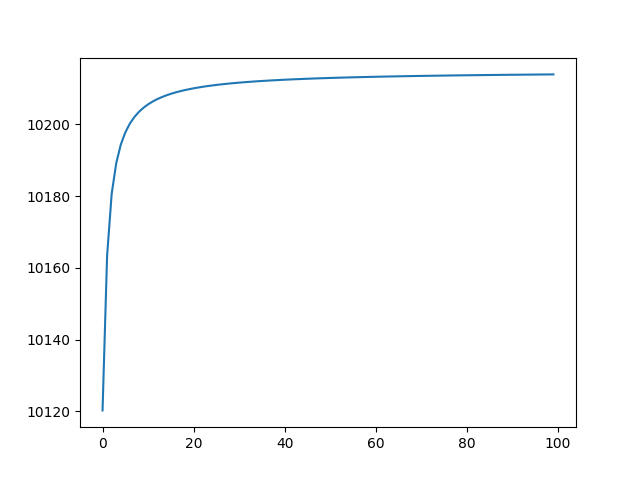
\includegraphics[scale=0.8]{plot/utility}
    \end{center}
    There appears to be convergence to a point near 10210 (2.1 readjusted).
    This is not necessarily joint optimality,
    but is supported by the next point.

    By observing whether the original generated texts use pronouns or noun phrases,
    we find a selection of the \Generator{}'s game choices.
    We can assume the \Resolver{} succeeds and calculate the utility.
    The total utitity is 10193 (1.93 readjusted).

    This is notable since the game performance for the language-based players
    that had full access to syntactic and semantic information
    performed slightly worse than the game theoretic players.

    This could be interpreted as a sign of an incorrect assumption in the game formulation,
    namely that humans prefer pronouns when they are unambiguous.
    Even when the pronouns are unambiguous,
    speakers may often choose to use nouns for the sake of fluidity,
    extra clarity, emphasis, or a number of other factors.

    It is much more likely that this is simply a case of overfitting.


    \section{Limitations}\label{sec:limitations}

    \begin{itemize}
        \item
        Even with the techniques applied to make the game space small, it is still slow to run,
        and can't be expanded further without a significant increase in computational power.

        \item
        As mentioned before,
        removing everything except the entities results in a significant loss of contextual information.
        For instance, the example sentence
        \begin{quote}
            \textbf{The students} saw \textit{the papers} on the floor, so \textbf{they} picked \textit{them} up.
        \end{quote}
        cannot be represented with the corresponding placeholders
        as [``students'', ``papers'', \Placeholder{}, \Placeholder{}]
        since the semantic context of ``picked \dots up'' as a verb that usually has an animate agent is lost.

        \item
        Similarly, using a bare \Placeholder{} conflates distinct pronouns.
        This is worth considering from a gameplay perspective since certain pronouns are
        more likely to be used for certain entities.
        However, it complicates the model for the same reason.

        \item
        Even when $S$ has linguistic structure,
        it may be the case that certain strategies dominate that do not use that structure.
        One possible way to address this could be by making the payout smaller for more frequent entities.
    \end{itemize}


    \section{Further Research}\label{sec:further-research}

    Similar techniques could be used to analyze a wide variety of linguistic patterns,
    including dependency parsing, translation word choice, and sentiment analysis.
    I think it is unlikely that it will ever outperform modern language models,
    but there may be some cases where the games are small enough
    and exhibit such suitable patterns that game solving techniques can
    be used alongside language models to account for some of their deficiencies.


    \section{Resources and Related Work}\label{sec:resources-and-related-work}

    \begin{itemize}
        \item
        \texttt{transformers} (\url{https://huggingface.co/docs/transformers/en/index})

        \item
        BLOOM Language Model (\url{https://bigscience.huggingface.co/blog/bloom})

        \item
        spaCy (\url{https://spacy.io/})

        \item
        \texttt{fastcoref} (\url{https://github.com/shon-otmazgin/fastcoref})

        \item
        ChatGPT (\url{https://chatgpt.com/})

        \item
        The Consensus Game: Language Model Generation Via Equilibrium Search
        (Jacob, Shen, Farina, Andreas)

        A two-player cooperative imperfect information game for a natural language task
        that served as inspiration for this one.
    \end{itemize}


\end{document}
